\item \points{25} {\bf Poisson Regression}

In this question we will construct another kind of a commonly used GLM, which is called Poisson Regression. In a GLM, the choice of the exponential family distribution is based on the kind of problem at hand. If we are solving a classification problem, then we use an exponential family distribution with support over discrete classes (such as Bernoulli, or Categorical). Simiarly, if the output is real valued, we can use Gaussian or Laplace (both are in the exponential family). Sometimes the desired output is to predict counts, for e.g., predicting the number of emails expected in a day, or the number of customers expected to enter a store in the next hour, etc. based on input features (also called covariates). You may recall that a probability distribution with support over integers (i.e. counts) is the Poisson distribution, and it also happens to be in the exponential family.

In the following sub-problems, we will start by showing that the Poisson distribution is in the exponential family, derive the functional form of the hypothesis, derive the update rules for training models, and finally using the provided dataset train a real model and make predictions on the test set.

\begin{enumerate}
	\item \subquestionpoints{5} Consider the Poisson distribution parameterized by
$\lambda$:
%
\begin{equation*}
  p(y; \lambda) = \frac{e^{-\lambda}\lambda^y}{y!}.
\end{equation*}
%
(Here $y$ has positive integer values and $y!$ is the factorial of $y$. ) 
Show that the Poisson distribution is in the exponential family, and
clearly state the values for $b(y)$, $\eta$, $T(y)$, and $a(\eta)$.


\ifnum\solutions=1{
  \begin{answer}
	Rewrite the distribution function as:
	\begin{eqnarray*}
		p(y;\lambda) &=& \frac{ e^{-\lambda} e^{y \log \lambda}}{y!}\\
		&=& \frac{1}{y!} \exp(y \log \lambda - \lambda)
	\end{eqnarray*}
	
	Comparing with the standard form for the exponential family:
	\begin{eqnarray*}
		b(y) &=& \frac{1}{y!}\\
		\eta &=& \log \lambda\\
		T(y) &=& y\\
		a(\eta) &=& e^\eta.
	\end{eqnarray*}
\end{answer}

}\fi

	\item \subquestionpoints{3} Consider performing regression using a GLM model
with a Poisson response variable.  What is the canonical response function for
the family?  (You may use the fact that a Poisson random variable with
parameter $\lambda$ has mean $\lambda$.)



\ifnum\solutions=1{
	\begin{answer}
	\begin{equation*}
	    g(\eta) = E[T(y);\eta] = E[y;\eta] = E[y; log(\lambda)]= \lambda = e^{\eta} = e^{\theta^{T}x}
	\end{equation*}
	
	Therefore, the canonical response function of Poisson distribution is $e^{\theta^{T}x}$
\end{answer}

}\fi

	\item \subquestionpoints{7} For a training set
$\{(x^{(i)}, y^{(i)});\, i=1,\ldots,\nexp\}$, let the log-likelihood of an example
be $\log p(y^{(i)} | x^{(i)}; \theta)$. By taking the derivative of the
log-likelihood with respect to $\theta_j$, derive the stochastic gradient
ascent update rule for learning using a GLM model with Poisson responses $y$
and the canonical response function.



\ifnum\solutions=1{
  \begin{answer}
The log-likelihood of an example $(x^{(i)}, y^{(i)})$ is defined as
$\ell(\theta) = \log p(y^{(i)} | x^{(i)}; \theta)$. To derive the stochastic
gradient ascent rule, use the results in part (a) and the standard GLM
assumption that $\eta = \theta^Tx$.
\begin{eqnarray*}
	\frac{\partial \ell(\theta)}{\partial \theta_j}
	&=& \frac{\partial \log p(y^{(i)} | x^{(i)}; \theta)}{\partial \theta_j}\\
	&=& \frac {\partial \log \left({\frac{1}{y^{(i)}!} \exp(\eta^T y^{(i)} -
	e^\eta)}\right)} {\partial \theta_j}\\
	&=& \frac {\partial \log \left(\exp((\theta^Tx^{(i)})^T y^{(i)} -
	e^{\theta^Tx^{(i)}})\right)} {\partial \theta_j}
	+ \frac {\partial \log \left({\frac{1}{y^{(i)}!}}\right)} {\partial
\theta_j}\\
	&=& \frac {\partial \left((\theta^Tx^{(i)})^T y^{(i)}
		- e^{\theta^Tx^{(i)}}\right)} {\partial \theta_j}\\
	&=& \frac {\partial \left((\sum_k \theta_k x^{(i)}_k) y^{(i)}
		- e^{\sum_k\theta_k x^{(i)}_k}\right)} {\partial \theta_j}\\
	&=& x^{(i)}_jy^{(i)} - e^{\sum_k \theta_k x^{(i)}_k} x^{(i)}_j\\
	&=& (y^{(i)} - e^{\theta^T x^{(i)}}) x^{(i)}_j.
\end{eqnarray*}

Thus the stochastic gradient ascent update rule should be:
%
\begin{equation*}
\theta_j := \theta_j + \alpha \frac{\partial \ell(\theta)}{\partial \theta_j},
\end{equation*}
%
which reduces here to:
\begin{equation*}
	\theta_j := \theta_j + \alpha (y^{(i)} - e^{\theta^T x^{(i)}}) x^{(i)}_j.
\end{equation*}
\end{answer}

}\fi

	\item \subquestionpoints{10} \textbf{Coding problem}

Consider a website that wants to predict its
daily traffic. The website owners have collected a dataset of past traffic to
their website, along with some features which they think are useful in
predicting the number of visitors per day. The dataset is split into
train/valid sets and the starter code is provided in the following files:
\begin{center}
\begin{itemize}
\item 	\url{src/poisson/{train,valid}.csv}
\item   \url{src/poisson/poisson.py}
\end{itemize}
\end{center}
We will apply Poisson regression to model the number of visitors per day.
Note that applying Poisson regression in particular assumes that the data
follows a Poisson distribution whose natural parameter is a linear
combination of the input features (\emph{i.e.,} $\eta = \theta^T x$).
In \texttt{src/poisson/poisson.py}, implement Poisson regression for this dataset
and use \emph{full batch gradient ascent} to maximize the log-likelihood of $\theta$. For the
stopping criterion, check if the change in parameters has a norm smaller than
a small value such as $10^{-5}$.

Using the trained model, predict the expected counts for the \textbf{validation set}, and
create a scatter plot between the true counts vs predicted counts (on the
validation set). In the scatter plot, let x-axis be the true count and y-axis
be the corresponding predicted expected count. Note that the true counts
are integers while the expected counts are generally real values.



\ifnum\solutions=1 {
  \begin{answer}
	\begin{figure}[H]
		\centering
		\vspace{-2mm}
		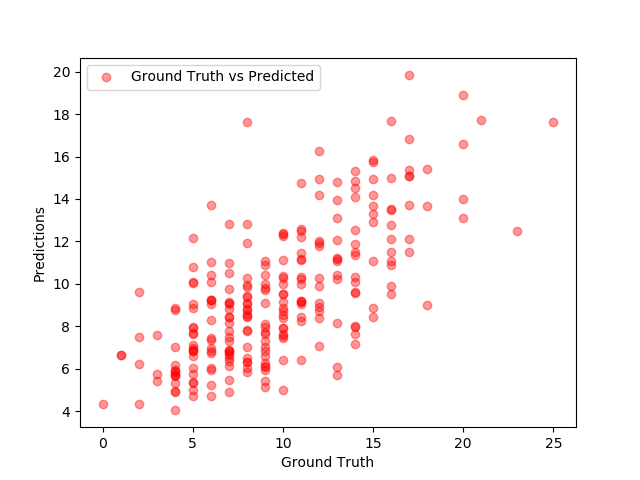
\includegraphics[width=0.65\linewidth]{../src/poisson/poisson_valid.png}
		\caption{Ground Truth vs Prediction plot on the validation set}
	\end{figure}


Note: Depending on the initial value of $\theta$, the final value of $\theta$ may be different. However, the log-likelihoods and predictions are nearly identical. This happens because of the way the data was simulated. $x_1$ is set to 0 or 1, and $x_2 = 1 - x_1$. Then, with the intercept term, $\theta_0 + \theta_1 x_1 + \theta_2 (1-x_1) = (\theta_0 + \theta_2) + (\theta_1 - \theta_2) x_1$. So we can only recover $(\theta_0 + \theta_2)$, $(\theta_1 - \theta_2)$, $\theta_3$, and $\theta_4$.

\end{answer}

} \fi

\end{enumerate}
